%========================================================
% File:         Resumes
% By:           Roberto Cantu Funes
% Date:        16/9/2018
% Modified:  xx
%========================================================
\documentclass[letterpaper,titlepage,11pt]{article}
\usepackage[left=2cm, right=2cm, top=2cm, bottom=2cm]{geometry}
\usepackage{setspace}
\onehalfspacing
\usepackage[utf8]{inputenc}
\usepackage[T1]{fontenc}

\usepackage{multirow}
\usepackage{array}
\usepackage{amssymb}
\usepackage{setspace}
\usepackage{amsmath}
\usepackage{comment}
\usepackage[round]{natbib}
\usepackage{algorithm}
\usepackage{algpseudocode}
\usepackage{color}
\usepackage{pifont}
\usepackage{rotating} % Rotating table
\usepackage{placeins}
\usepackage{tabularx}

%
%       Text dimensions.
%

\hbadness=99999
\hfuzz=50pt

%commands
\newcommand{\cmark}{\ding{51}}
\newcommand{\true}{\textbf{True}}
\newcommand{\false}{\textbf{False}}
\newcommand{\citeAY}[1]{\citeauthor{#1}~(\citeyear{#1})}
\newcommand{\ltab}[1]{%
\makebox[.10\linewidth][l]{#1}\ignorespaces%
}%
\newcommand{\lftab}[1]{%
\makebox[.50\linewidth][l]{#1}\ignorespaces%
}%

%
%  Document starts here
%
\begin{document}

\thispagestyle{plain}
\begin{center}
    \Large
    Proposition de projet\\
    \textbf{Optimal Modulation Format Prediction for Physical Layer Network Planning}
 
    \vspace{0.4cm}
    \large
    Équipe 20
 
    \vspace{0.4cm}
    \textbf{Roberto Cantu Funes \qquad Allyson Fernandes Da Costa Silva}\\
    \textbf{Rizan Homayoun Nejad \qquad Hugo Siqueira Gomes}
 
    \vspace{0.9cm}
    \textbf{Abstract}
\end{center}

\section{Abstract}
Over the past decade, optical networks have been growing ‘smart’ with the introduction of software defined networking, coherent transmission and flexible grid. To name only few arising 23 technical and technological directions. The combined progress towards high-performance hardware and intelligent software, integrated through an SDN platform provides a solid base for promising innovations in optical networking. Machine learning algorithms can make use of the large quantity of data available from network monitoring elements to make them ‘learn’ from experience and make the networks more agile and adaptive. In this project, which is proposed and strongly advised by Professor Leslie Rusch at the \textit{Centre d'optique, photonique et laser} (COPL), Laval University, we focus on employing machine learning methods in optical networks to predict data transmission quality and identity the best possible capacity for a given configuration to improve the network's resource utilization.

\section{Introduction}
For decades, optical networks have provided larger bandwidths than could be utilized but today's telecommunication networks have become sources of enormous amounts of widely heterogeneous data. This information can be retrieved from network traffic traces, network alarms, signal quality indicators, users' behavioral data, etc. With this increasing growth of the global Internet traffic demand, new optical transmission technologies are required to provide a much higher data rate per channel and to enable more flexibility in the allocation of traffic flow. Software-defined networking (SDN) is an architecture that aims to make networks flexible. The goal of SDN is to improve network control by enabling service providers to respond quickly to changing business requirements. Basically, it uses software applications to be intelligently programmed. As a result, we can consistently manage the entire network. In this regard, advanced mathematical tools are required to extract meaningful information from these data and take decisions related to the proper functioning of the networks from the network generated data. Among these mathematical tools, Machine Learning (ML) is one of the most promising methodological approaches to perform network-data analysis and enable automated network self-configuration. Among various networking areas, in this project, we focus on ML for optical networking. The adoption of ML techniques in the field of optical communication networks is motivated by the unprecedented growth of network complexity in the last few years. Such complexity increase is due to the introduction of a huge number of adjustable and interdependent system parameters (e.g., routing configurations, modulation format (capacity), symbol rate, coding schemes, etc.) that are enabled by the usage of transmission/reception technologies, advanced digital signal processing and compensation of nonlinear effects in optical fiber propagation
Optical networks constitute the basic physical infrastructure of all large-provider networks worldwide, thanks to their high capacity, low cost and many other properties and there is no sign that a substitute technology might appear in the foreseeable future. In fact, ML application can be useful especially in cross-layer settings, where data analysis at physical layer, e.g., monitoring Bit Error Rate (BER), can trigger changes at network layer, e.g., in routing, spectrum and modulation format assignments. The application of ML to optical communication and networking is still in its infancy. It is currently perceived as a paradigm shift for the design of future optical networks and systems. These techniques should allow to infer from data useful characteristics that could not be easily or directly measured.
The application of ML to physical layer use cases is mainly motivated by the presence of non-linear effects in optical fibers, which make analytic models inaccurate or even too complex. This has implications on the performance predictions of optical communication systems, in terms of Bit-Error-Rate (BER), quality factor (Q-factor) and also for signal demodulation. Several challenges need to be addressed at the physical layer of an optical network, typically to evaluate the performance of the transmission system and to check if any signal degradation influences existing lightpaths. Such monitoring can be used, e.g., to trigger proactive procedures by varying modulation format before signal degradation occurs.

\section{Modulation format recognition (MFR)}
Modern optical transmitters and receivers provide high flexibility in the utilized bandwidth, carrier frequency and modulation format, mainly to adapt the transmission to the required bit-rate and optical reach in a flexible networking environment. Given that at the transmission side an arbitrary coherent optical modulation format can be adopted, knowing this decision in advance also at the receiver side is not always possible, and this may affect proper signal demodulation and, consequently, signal processing and detection. Using ML algorithms can help the modulation format recognition at the receiver, thanks to the opportunity to learn the mapping between the adopted modulation format and the features of the incoming optical signal. Researchers have already started exploring the application of machine learning algorithms to enable smart optical networks. In this case, ML can be employed to build data-driven models for more accurate and optimized network provisioning and management. In this project we aim to attack this problem and predict the optimum modulation format (best capacity) for sending the data based on input features. In this case, we will use a training dataset with a size of 60000, and we have all the training data we need which is generated by an optical setup. The figure below shows our optical links for our dataset; at its transmitter side, we will have several features and at the receiver, we will have one output which is our capacity that we want to predict. The list of input and output features for our case study is shown in the picture. As can be seen, there are 11 input features affecting our problem. As a first step, we aim to reproduce the results from \citep{rafique2018machine}, which used a MLP algorithm to predict the output using different number of layers and neurons and reported the results based on classification accuracy and training time, And then identify and choose the most important features affecting the results, and Finally apply other ML methods and compare it to the published results in terms of accuracy, complexity and efficiency.
\begin{center}
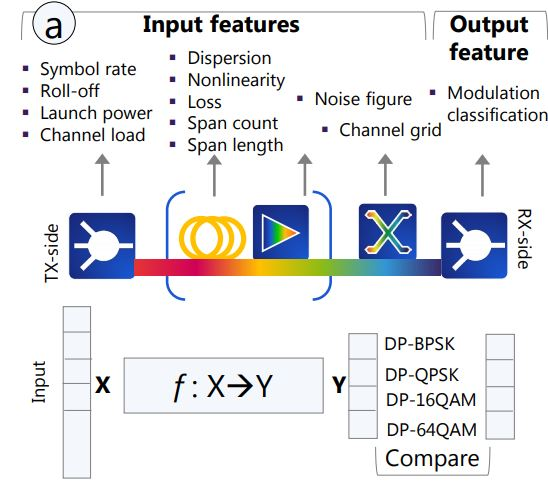
\includegraphics[scale = 1]{img1.JPG}
\end{center}

%   References
%
\bibliographystyle{plainnat}
\bibliography{refs}

\end{document}


